%\documentclass{article}
%\usepackage{graphicx,subfigure}
%\begin{document}

\begin{figure}[!h]
  \centering
  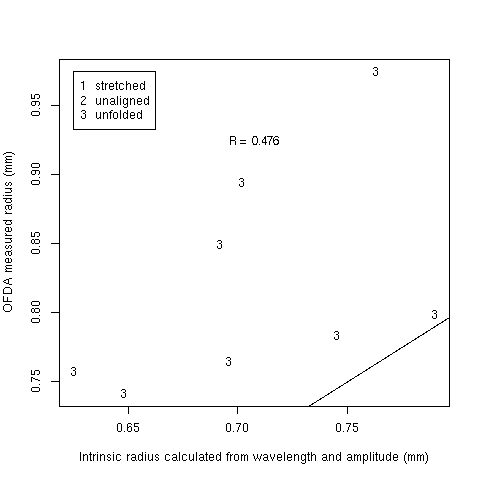
\includegraphics[width=1.0\textwidth]{figwaradthetaunfoldsf.png}
%   figwaradthetaunfoldsf.png is original 
  \caption{Intrinsic radius of curvature calculated from wavelength and amplitude measured by the SF technique, plotted against OFDA measured radius of curvature for unfolded wools only. Each point is a sheep mean.}
  \label{fig:waradthetaunfoldsf}
\end{figure}

%\end{document}

